\section{Implementation}
\label{chapter:implementation}
\label{sec:implementation}
	% Chapter concerning the Technical Realization

	In this chapter we will deal with the infrastructure and technical realization of the public display survey platform. First, the requirements for the survey platform are discussed (section \ref{sec:implementation:requirements}). Subsequently the architecture resulting from the design decisions will be the main focus (section \ref{sec:implementation:design-decisions}). To facilitate the training period for successors we will also take a brief look at the software model (section \ref{sec:implementation:modeling}). For more specific information and for information regarding maintenance of the project, please refer to the documentation found on the CD enclosed or on the GitHub repository (see Appendix \ref{appendix:documentation}).

	In figure \ref{fig:4-pdsurvey-platform} a brief overview of the PDSurvey platform and its components is given. The platform consists of three major parts: a backend for display providers (PDAdmin), a RESTful server (PDServer) and the user interface itself, being embedded on the end user devices (public displays, tablets, smartphones or other devices). 





\subsection{Requirements}
\label{sec:implementation:requirements}

	The starting point for the PDSurvey platform, and the Master's thesis itself, was the official announcement\footnote{\url{http://www.medien.ifi.lmu.de/lehre/arbeiten/detail.xhtml-php?pub=alt_pdsurvey} (last visited on March 24, 2015)}, describing the scope of the thesis. This problem statement already included first requirements for the survey platform to develop, and was also a trigger for further literature review and talks with people from the industry.

	% Official Problem statement
	\begin{enumerate}[itemsep=0pt] 
	\item \textit{development of a survey tool} that allows interactive public display installations to be comprehensively assessed 
	\item a web-based survey platform will be implemented that can easily be used to evaluate and compare public displays through \textit{different channels} 
	\item \textit{different channels} to support: 1) evaluation directly at
	the display or 2) through a (mobile) website that allows participation via smartphone or tablet.
	\item \textit{configuration options} for public display owners
	\end{enumerate}

	Additional requirements, that have emerged during research and in discussions, are listed below:

	% Derived requirements
	\begin{itemize}[itemsep=0pt] 
	\item easy \textit{embedding of questionnaires} on websites of public display owners (provide API / embed code)
	\item support \textit{various devices}: public displays of all sizes, tablets, phablets, smartphones, desktop devices (responsive web design)
	\item allow for both \textit{quantitative and qualitative} metods of data collection
	\item easy \textit{scalability} of platform, host on a cloud platform
	\item use a \textit{modular approach}, allowing successors to extend and further refine the platform
	\item focus on \textit{public display evaluation}, take the context into account for evaluation
	\item furthermore design guidelines for the construction of public display applications introduced by Huang et al. \cite{huang2008overcoming} and Jacucci et al. \cite{jacucci2010worldsofinformation} were followed.
	\end{itemize}

	These requirements combined with knowledge from literature review, are what makes this platform unique. The long term goal is to create a research platform, optimized for public display evaluation, delivering new insights into how users react to public display setups. All of the mentioned requirements had an impact on the chosen architecture, will be discussed in the next section.



\subsection{Design Decisions}
\label{sec:implementation:design-decisions}

	After having assessed all requirements for the platform (see section \ref{sec:implementation:requirements}), the next step was making design decisions for the software, programming language and frameworks to use, before starting with the practical implementation of the platform. 

	Two weeks were taken for assessing all of the possibilities, on the one hand to get informed what is currently buzzing, on the other hand because every decision made has an impact on the architecture. Changing a technology half way through the project is not an option for the duration of this Master thesis.


	\paragraph{Programming language}

		Due to the requirements and objective to support a large number of devices, operating systems, and form factors, a device-independent programming language was preferred. 
		The choice fell on Javascript, not just due to the growing popularity\footnote{\url{http://www.sitepoint.com/javascript-internet-things/} (last visited on November 27, 2014)}, but also because it can be used on the largest number of platforms and devices. Another huge benefit is being able to only use JavaScript for all tiers of development, from client to server to persistence layer. Using the same language on all tiers allows us to share some parts of code between server and client. This approach has become very popular in recent years, now often being being encapsulated in a technology stack referred to as the MEAN stack, consisting of MongoDB, Express.js, Angular.js, and Node.js. Some fundamental differences to the LAMP stack (Linux, Apache, MySQL, PHP) are its shift form server-side to client-side single-page applications (SPA), faster prototyping, shift from synchronous to asynchronous, fast page loading times, less time spent writing SQL (schemaless), and the shift to using RESTful services for the backend\footnote{\url{http://www.ibm.com/developerworks/library/wa-mean1/index.html} (last visited on March 26, 2015)}. This already led for the first time to the thought of choosing the MEAN stack\footnote{\url{http://mean.io/} (last visited on March 26, 2015)} for the entire development. Nonetheless each part of the architecture was compared and evaluated separately, in order to find the optimal solution for this project.

		Alternative languages considered were: PHP, Python, Ruby, Java and ASP.NET. The biggest drawback was the additional workload on having to maintain the object model on multiple platforms. With Javascript it is possible to only having to maintain the object model once, easily keeping it consistent across all platforms (backend, frontend, server).

		Based on our requirements for the platform, the feedback received from discussions with industry experts, and the desire to be able to embed questionnaires on 3rd party website, the choice to use JavaScript for the whole development process already became evident. The still open question was whether to fully go along with the MEAN stack, or if it makes sense to replace Angular.js, Express.js or MongoDB with another solution..


	\paragraph{Frontend}

		The next question to be answered was which technologies to use in the frontend, leading to the question whether to follow the single-page application approach or not. As of 2014 JavaScript model-view frameworks most frequently used for creating single-page apps, are Angular.js, Ember.js and Backbone.js. When looking at the numbers and the trend from recent years, Angular.js is the clear favorite. It has by far the largest user base on GitHub, Stackoverflow, and Youtube. When comparing the number of third-party modules, Angular.js also takes the lead with 800 ngmodules vs. 236 Backbone.js backplugs vs. 21 emberaddons\footnote{\url{https://www.airpair.com/js/javascript-framework-comparison} (last visited on January 11, 2015)}. All these factors together indicate a short training time and give hope for making fast progress as beginners. 
		One of the biggest benefits of using a framework like Angular.js, is the ability to use two-way data-binding. Changes made to the model are automatically represented in the UI, and vice versa. Furthermore, the possibility to use the templating functionality, combined with the custom directives in Angular.js, was a big plus for this choice. This functionality was used for creating custom HTML tags for the question types in our surveys. These were amongst other the reasons why we chose Angular.js for this project, hoping that it will also simplify the ramp-up time for other students.

		To speed up frontend development we chose Bootstrap\footnote{\url{http://getbootstrap.com/} (last visited on December 1, 2014)} as our CSS framework of choice. Reasons for choosing Bootstrap were the large community, extensive documentation with helpful examples, large number of free tutorials and templates, its excellent integration with Angular.js (AngulatStrap\footnote{\url{http://mgcrea.github.io/angular-strap/}} and AngularUI), the short training time, and because it is so well established.
		Alternatives considered were Foundation Framework by Zurb, however at the time of writing there was no prefabricated integration for Foundation and Angular.js.
		A good overview\footnote{\url{http://www.sitepoint.com/5-most-popular-frontend-frameworks-compared/} (last visited on December 2, 2014)} and a comparison\footnote{\url{http://www.sitepoint.com/grid-system-comparison-bootstrap-vs-foundation/} (accessed March 24, 2015)} of currently popular frontend frameworks was also considered.
	

	\paragraph{Backend}

		For the backend it was most important to have a solid and scalable solution with good performance, since our system might need to scale in the future, having a multiplicity of clients attached to the survey platform, all submitting responses and querying for different questionnaires. Additionally, it was of importance to offer an interface for administrators and to easily be able to exchange data with a large number of clients. For this reason a backend built solely on the principles of a RESTful API was preferred, being able to query the data from no matter which platform.
		% get curve to MEAN, say why we chose it now
		Based on the decision to use JavaScript for all tiers, it was also clear to use Node.js as the underlying platform for building web applications. Reasons speaking for Node.js are its event-based and modular approach, only requiring the parts needed for your project. Another benefit is the easy implementation of authentication or internationalization, due to the concept of middlewares \footnote{\url{http://www.heise.de/developer/artikel/REST-Webservices-mit-Node-js-Teil-1-Connect-als-Fundament-1802258.html?view=print} (last visited on November 24, 2014)} and the native serialization of JSON. Furthermore it is great for reusing code, due to its modular and lightweight architecture and the npm package manager \footnote{\url{http://www.heise.de/developer/artikel/2x-Nein-4x-Ja-Szenarien-fuer-Node-js-2111050.html} and \url{http://stackoverflow.com/questions/5062614/how-to-decide-when-to-use-node-js} (both last accessed on April 9, 2015)}. To simplify and speed up development with Node.js, Express.js\footnote{\url{http://expressjs.com/} (last accessed on April 10, 2015)} was chosen as the web application framework. Alternatives considered were Connect (simpler, less functionality, predecessor of Express), Koa\footnote{\url{http://koajs.com/} (last accessed on April 10, 2015)} (generator concept) and Resitfy\footnote{\url{http://mcavage.me/node-restify/} (last accessed on April 10, 2015)} (Express reduced for pure REST services). 

		% Communication: RESTful interaction
		Due to the decision to build a single-page application, it became vital to separate the data from presentation layer. Using a RESTful service is the current de facto standard. An alternative would be to use SOAP for message exchange. This would not only lead to an increase of data overhead, but also to a higher complexity on the server-side, and to the loss of statelessness in the requests. Should a client not support HTML or JavaScript execution, then the required surveys can still be requested directly with the REST API through rudimentary HTTP function calls, being another benefit for implementing a RESTful API.

		Such an exception was Quest3D\footnote{\url{http://documentation.quest3d.com/index.php?title=FAQ\#What_is_Quest3D.3F} (last accessed on April 10, 2015)}, a software package used by Jiamin Shi for the development of the Balloon Shooter game. When being in a situation where HTTP calls are not supported natively, then one can still use logging combined with a scheduled task or create a proxy on the operating system layer and tunnel all data to the PDServer.





	\paragraph{Database}

		Another fundamental aspect presented the question where to store the data persistently. Criteria for choosing the right database management system (DBMS) for this project were again the size of community, suitability for prototyping, and ease of integration with Node.js/Angular.js. The first question presented, was whether to choose a SQL or a NoSQL DBMS. We chose NoSQL for this project, because better scalability, a schemaless data representation, faster response time and a decreased development time\cite{vaish2013getting}. Otherwise, NoSQL is better suited for rapid prototyping, because multiple schema can be mixed inside of one collection and easier evolve over time. These are all arguments speaking for using a NoSQL DBMS for our scenario. 

		Out of the NoSQL databases MondoDB\footnote{\url{http://www.mongodb.org/}} represents the most popular DBMS, especially since it integrates seamlessly into the MEAN stack. Benefits of MongoDB are being non-relational (and schemaless), plus its ability to directly store JavaScript object inside the database, being the biggest advantage. Other characteristics of MongoDB are the non-blocking write operations, being ideal for logging data. MongoDB provides a good compromise between scalability/performance and the depth of functionality. One disadvantage is that MongoDB does not support joins or transactions. For our use case, however, this is no major drawback. The benefits outweigh the disadvantages. 

		Alternatives looked at were CouchDB and Redis. Redis being useful for fast changing data, which is not the case for our platform. CouchDB would be an alternative worth looking at, having a better replication and conflict resolution. This additional security is however not needed. The speed benefits of MongoDB are preferred.\footnote{\url{http://kkovacs.eu/cassandra-vs-mongodb-vs-couchdb-vs-redis} (accessed March 26, 2015)}

		To facilitate the object modeling process in Node.js, Mongoose\footnote{\url{http://mongoosejs.com/} (accessed November 14, 2014)} was chosen, providing object relational mapping. Mongoose is an object modeling package for Node.js, allowing to application data to be modeled based on schemata. Mongoose takes care of performing CRUD applications and simplifies keeping the object model synchronized across all layers.


	\paragraph{Hosting}

		For the hosting of the platform a free and easy scalable solution was of importance. Services offering a platform as a service (PaaS) were preferred over ones offering a infrastructure as a service (IaaS), because our focus currently is on developing and evaluating the platform. We considered the following platforms: Heroku (PaaS), IBM BlueMix (PaaS), Amazon AWS (IaaS), or hosting the entire platform on a local machine.

		Our first choice was Heroku\footnote{https://www.heroku.com/}, due to its simplicity of setup, its native support of Node.js and the seamless integration with Mongolab\footnote{https://mongolab.com/}, a platform for hosting MongoDB collections.
		Alternatives considered were Google App Engine, IBM BlueMix, Amazon Web Services (Amazon EC2) or hosting everything on local machines at our university. However for our scenario all of the above options had their drawbacks in comparison to Heroku. Google App Engine (as of December 2014) still had no native support for Node.js and custom runtimes had to be used to get Node.js support up and running. IBM BlueMix just got overhauled, offered full out-of-the-box Node.js support, however they only the first 30 days were free and the pricing model wasn't as attractive. Amazon Web Services offering a Infrastructure as a Service (IaaS), would have required too much administration of the server, which would have slowed down the main objective of the project, the development of the survey platform\footnote{\url{http://smashingboxes.com/ideas/heroku-vs-amazon-web-services} (last accessed on April 10, 2015)}. The same goes for the last option, hosting a MEAN-stack environment on our own servers at LMU Munich. All of the above are well-known solutions in the industry, however due to simplicity and ease of use we chose Heroku. For our requirements during the prototype phase Heroku was sufficient, offering one free Heroku \textit{dyno}\footnote{\url{https://devcenter.heroku.com/articles/how-heroku-works\#running-applications-on-dynos} (last accessed on April 10, 2015)}.



		\paragraph{MEAN Stack}
		As already predicted in the beginning, we ended up using the full MEAN stack for developing PDSurvey. The clear benefit is the ability to use JavaScript from client to server to persistence level. Scott Davis has published a good article on ibm.com with an introduction to the MEAN stack and a short recap of the last ten years of web development\cite{Scott2014MEANStack}.






\clearpage

\subsection{Modeling}
\label{sec:implementation:modeling}

	The development process of the PDSurvey platform was inspired and influenced by the concept of extreme programing\footnote{\url{http://www.extremeprogramming.org/rules.html} (last visited on April 10, 2015)}, making iterative improvements, and working agile and user centered. First user stories were written and assessed in a small group\footnote{\url{http://www.tigertech.de/wie-schreibe-ich-eine-gute-user-story-und-was-ist-das-uberhaupt/} (last accessed April 10, 2015)}. The next step was to transfer these stories to user models, describing in detail which functionality the stakeholders of PDSurvey are supposed to have. Later a first software architecture and software model was built. Dependencies between models were defined and the model was continuously refined and improved throughout the development phase. The last phase included screen designs, getting a clear view of what the interface might later look like.

	% Mongoose + REST API
	The model for the \textit{PDSurvey} platform is maintained with Mongoose. Angular.js builds its model from the REST API, and maps all changes via dynamic two-way-binding to it's scope. The REST API is provided by the Node.js server, which maps all incoming requests through an Express router to the corresponding Mongoose models. Thus all changes to the model originate from Mongoose.

	% User roles
	Currently three user roles are implemented for the platform: an \textit{admin} role (for administrators), an \textit{expert} mode (with a mapping of n surveys to m displays), and a \textit{novice} mode (with a simplified interface).

	% REST API
	The development of the REST API was influenced by current best practices \cite{Sahni2015RESTAPI, TutsPlus2015RESTAPI, hughes2012einfuhrung}. The API is separated into logical resources, while each resource gets manipulated through an HTTP request. For public access GET and POST is defined, for authenticated users also PUT and DELETE. For a more information about PDSurvey's REST API refer to the documentation (see Appendix \ref{appendix:documentation}).

	% Our Software Model
	The software model is modeled in Mongoose and stored as MongoDB collections. There are the following collections: \textit{Question, QuestionType, Response, Category, Surveys, User, DisplayModel, Display, Campaign, Context, User}. 
	Of special interest are the following four collections: Surveys, Display, Campaign and Responses (see figure \ref{fig:4-dependency-campaign}).

\begin{figure}%[btph]
    \begin{center}
        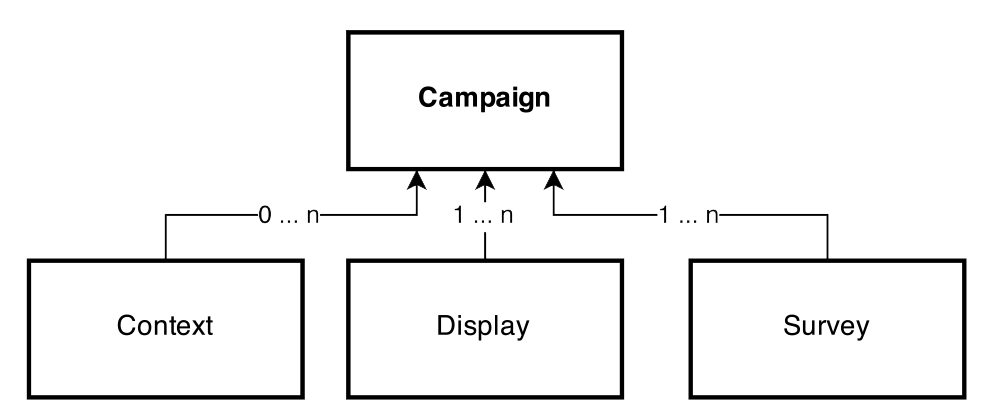
\includegraphics[width=.8\columnwidth]{img/4_implementation/4-dependency-campaign}
    \end{center}
 % \begin{center}\LARGE [BILD]\end{center}
 \caption{Campaign model dependencies}
 \label{fig:4-dependency-campaign}
\end{figure}


	\paragraph{Surveys:} Questionnaires are the foundation of PDSurvey, consisting of multiple sections, which in turn are made up of multiple questions. Each question is of a corresponding question type and every questionnaire belongs to a category. This allows questionnaires to be filtered based on certain research questions. Additionally we added the ability to set surveys \textit{private} (by default), \textit{shared} (for sharing with other users), \textit{standardized} (scientifically recognized), or \textit{pending} (waiting for review, to be shared). Every survey is assigned to an individual user of the platform, with the aim of reuse and standardization of questionnaires.

	\textbf{TODO ueberlegen ob ich den letzten Absatz Surveys oder Questionnaires nennen mag}


	\paragraph{Display:} In the display collection all displays connected to the PDSurvey platform are contained. To allow for an evaluation across multiple display models and based on the context of the displays, the display model and a static and/or dynamic context is assigned to it.

	\paragraph{Campaign:} Campaigns resemble the most integral part of the platform, since they glue all of the pieces together and allow the distribution of surveys to public display networks. A campaign consists of displays and surveys, and creates the mapping of the questionnaires to public displays. Additionally to each of those mapping an individual context can be assigned, enabling the later comparison of results in between the public displays.

	\paragraph{Response:} All responses made to each survey are logged in the Response collection. The queries are logged individually per user, per display and per campaign. This model will be the base for further extensions, such as the automatic evaluation of the survey responses and the comparison in between different displays inside one display network. This enables to find out which properties of a display might cause certain effects.

	\paragraph{Context:} One of the benefits of creating this survey platform is the ability to collect and evaluate large amounts of data, without increasing the workload on the human component for conducting and evaluating the responses. The idea is to collect a large number of responses from a variety of displays in various settings, and assigning a specific context to every display connected to PDSurvey. Once enough data is collected, the results can be evaluated and compared in between the displays. Interesting questions for analysis would be, which role the context plays on how the users respond to the display, when running identical software settings on the displays, but only varying the context (position, size of display, surrounding environment of the display, positioning it outdoors or indoors, influence of the weather, type of building it is positioned in).



